\section{Use Cases}

\begin{enumerate}
  \item students can manage and view all details related to their enrollment and coursework   
  \item Students can choose courses to be enrolled in.
  \item Students must pay the enrollment fees after qualified to enroll.
  \item System admin lists the courses and eligibility criteria for each course.
  \item System admin permits students to edit user data.
  \item System admin verifies student  criteria are met, then decides to approve or cancel the enrollment.
  \item Tutors are assigned to the candidate
  \item Students get to see their course and Tutors assigned.
  \item Tutors can view the students for whom they will be conducting the courses
\end{enumerate}

\begin{figure}[hbt!]
    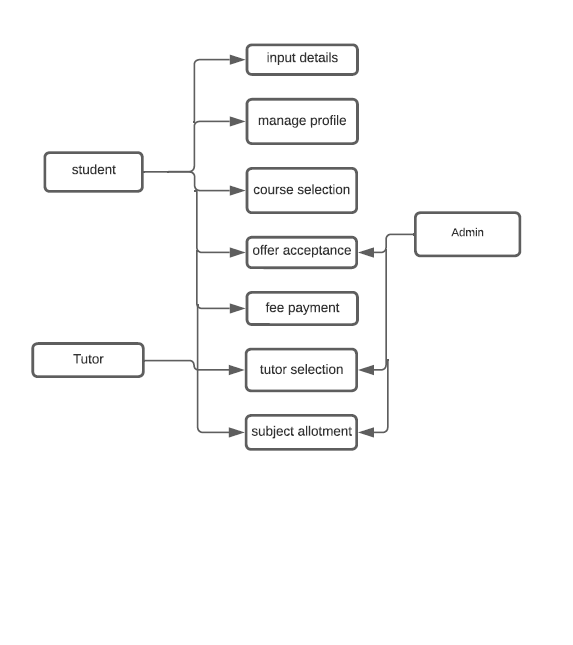
\includegraphics{1.png}
    \caption{Use Case Diagram}
\end{figure}







\begin{table}[]
\begin{tabular}{@{}|c|c|c|c|c|@{}}
\toprule
use case                & actor   & description                                                   & condition                                     & trigger                                                   \\ \midrule
fill Details            & Student & should create a profile and fill required information         & all basic qualifiations are met               & clikc on register                                         \\ \midrule
Choose course           & Student & During registration the required course is chosen             & eligible for the programme                    & selecting course from dropdown list                       \\ \midrule
Edit details permission & Admin   & Changes to student profile is authorized upon request         & A profile for the candidate is created        & editing request is raised                                 \\ \midrule
Edit details            & Student & Make changes to profile submitted for registration            & profile and course selection is completed     & Student chooses edit account                              \\ \midrule
Fee Payment             & Student & Students are able to pay the fee required for the course work & Course registration is approved               & fee payment is chosen                                     \\ \midrule
Assign course to tutor  & Admin   & Tutors are assigned to their respective courses               & Tutor is qualified to take-up the course      & Assign tutor when course has reached its minimum capacity \\ \midrule
Enrollment decision     & Admin   & The Admin decides if a student is eleigible or not            & The candidate profile passes all requirements & profile is created and submitted                          \\ \bottomrule
\end{tabular}
\end{table}
